As can be seen in Figure \ref{fig:cambresult}, we indeed observe a time-lagged movement of the Socialist centroids for each decade in the same direction as Marx's, namely, in the direction moving away from the Hegelian centroid and towards the political-economic centroid, from 1840 onwards (interestingly, after a move \textit{towards} the Hegelian centroid between 1830 and 1840).

\begin{figure}[ht!]
    \centering
    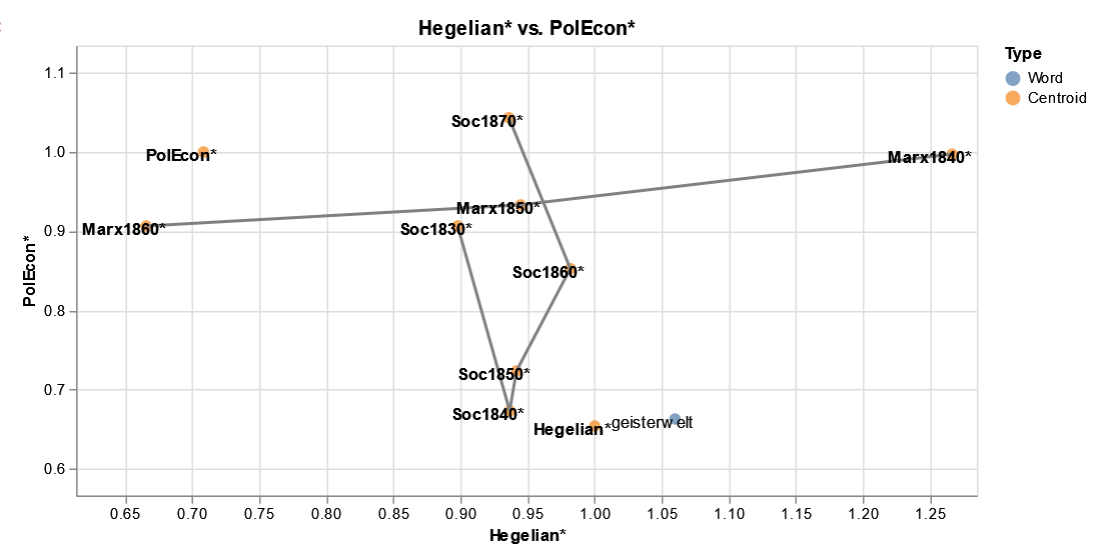
\includegraphics[width=\textwidth]{camb_result.png}
    \caption{The trajectories of Marx's decade-by-decade centroids and the decade-by-decade centroids of European socialist discourse, with respect to the static Hegelian (defining the x-axis) and Political-Economic (defining the y-axis) centroids.}
    \label{fig:cambresult}
\end{figure}

\begin{figure}[ht!]
\centering
\includesvg[width=\textwidth]{rolling_pe_sim.svg}
\caption{Rolling PE Similarity Scores for Marx's Collected Writings}
\end{figure}

\begin{figure}[ht!]
  \centering
  \includesvg[width=\textwidth]{pe_centroid.svg}
  \caption{A Principal Component Analysis (PCA) plot of the Political Economy centroid with the top $N = 25$ words most distinctive to this subcorpus.}
  \label{fig:pecentroid}
\end{figure}

\begin{figure}[ht!]
  \centering
  \includesvg[width=\textwidth]{heg_centroid.svg}
  \caption{A Principal Component Analysis (PCA) plot of the Hegelian centroid with the top $N = 25$ words most distinctive to this subcorpus.}
  \label{fig:hegcentroid}
\end{figure}

\begin{figure}[ht!]
  \centering
  \includesvg[width=\textwidth]{comb_centroid.svg}
  \caption{A plot of the two centroids used to define the ideological subspace (Political Economy and Hegelian), along with the top $N = 25$ words most distinctive to either subcorpus.}
  \label{fig:combcentroid}
\end{figure}
